\section{Background}
\label{sec:background}

\subsection{Library Learning and Abstract Syntax Trees}
Library extraction involves identifying and extracting the repeated functionalities from a corpus of programs, which is facilitated by analyzing the Abstract Syntax Trees (ASTs) of the programs. ASTs provide a structured representation of the code syntax, allowing algorithms to identify common patterns or partial sub-trees that can be abstracted into reusable functions. Consider a corpus of programs where multiple programs contain a similar sequence of operations to print a sum of two things as shown on the left side of Figure~\ref{figure:LibAbsAST}. The library extraction process could identify this common pattern in the ASTs of these programs and abstract it into a reusable function \texttt{print\_add(n)}. 



\begin{figure}[h]
  \centering
  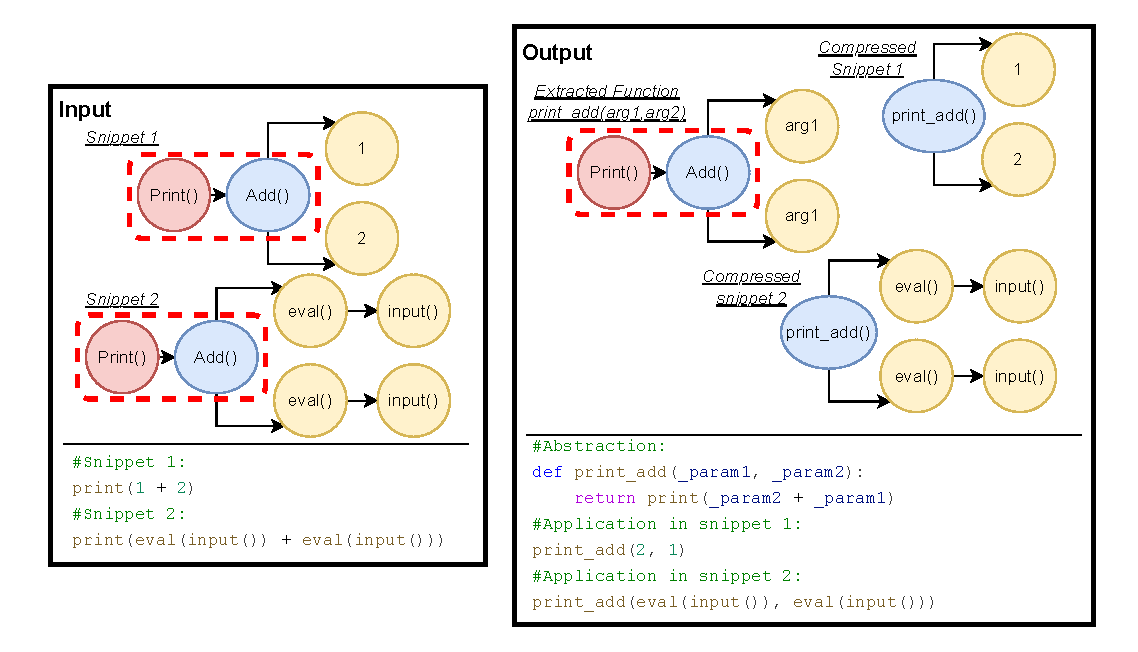
\includegraphics[width=\linewidth]{images/LibAbsAST.pdf}
  \caption{A library extraction example showing snippets of the input code, the output code, and their ASTs. The corpus (left) comprises of two code snippets who share a common structure (highlighted). CTS can extract this common structure, here named $print_add(arg1,arg2)$, and replace it with a function call (right).  }
  \todo{align image tops, move code comments to the side to compress vertically}
  \label{figure:LibAbsAST}
\end{figure}

\subsection{Corpus Guided Top-down Search}
Corpus Guided Top-Down Search (CTS) is a recursive search method~\cite{Bowers_2023stitch} that looks for the optimal function, with respect to some utility measure, to be extracted from a given corpus. The algorithm starts with the search target of a partial program tree, naively an empty tree, and it searches the corpus for matching partial sub-trees. The target's utility is then computed based on the number of matches found and the target's size, where larger targets with more matches have higher utility. In each subsequent round, the target is updated by adding child nodes to its leaf nodes. This expands the target, but consequently reduces the matches. The children are added depending on the corpus, as well as the expected utility. That is, the utility of expanding some branches of the target can be bounded by the current optimal utility, which guides the search to expand the target elsewhere. The search is concluded when the target reaches the optimal utility. The target then becomes the body of the extracted function, and the leaf's left-out children become the function's arguments. Figure \ref{figure:LibAbsAST} shows an example of CTS function extraction.  % JI: why left-out?  do we just mean the target's children?

% Top-down search starts with a small incomplete program, na
% Stitch extracts a library from a given program corpus by performing a corpus-guided top-down search (CTS) over the program's AST to find the optimal repeated sub-trees. In CTS, the search starts from the top with an empty program.  anwhere some AST nodes are included but their children are not. The omitted children represent search holes to be filled.\todo{explain the hole/topdown search thing 41:4,5} Stitch speeds up the library abstraction process by doing a utility-based CTS where it computes the utility of common sub-trees, and prune the search space to eliminate search paths that are guaranteed to have a lower utility than the current optimal one. The abstraction utility is calculated based on the size of the abstracted sub-tree and its useage frequency. Meaning abstracting complex functionalities that are more frequently used in the given corpus is prioritized over abstracting smaller ones or ones not frequently used. 
% }

% DreamCoder~\cite{ellis2020dreamcoder} is a State-of-the-art program synthesizer where the agent ( the synthesizer) is given a corpus of programs to learn from. Instead of synthesizing code directly, the agent first abstracts a library of repeated functionalities over the given corpus thus compressing the corpus. This reduces the agent's error probabilities by reducing the size of the code the agent has to write, as it can use the abstracted functions instead of rewriting them whenever needed. Hence, to speed-up program synthesis, one could speed up library abstraction. Library extraction involves identifying and extracting the repeated functionalities from a corpus, which is facilitated by analyzing the Abstract Syntax Trees (ASTs) of the programs. ASTs provide a structured representation of the code, allowing algorithms to identify common patterns or sub-trees that can be abstracted into reusable functions. Stitch~\cite{Bowers_2023stitch} is a State-of-The-Art library abstraction tool that takes in a list of programs written in a lisp-like syntax and outputs a library (a list of abstracted functions) while also re-writing the input programs to utilize the abstracted functions. It does so by performing a corpus-guided top-down search (CTS) over the programs' Abstract Syntax Trees (ASTs) to find the optimal repeated sub-trees. ASTs provide a structured representation of the code, allowing algorithms to identify common patterns or sub-trees that can be abstracted into reusable functions. Consider a corpus of programs where multiple programs contain a similar sequence of operations to compute the factorial of a number. The library extraction process would identify this common pattern in the ASTs of these programs and abstract it into a reusable function \texttt{compute\_factorial(n)}. Stitch speeds up the library abstraction process by doing a utility-based CTS where it computes the utility of found common sub-trees, and prune the search space to eliminate search paths that are guaranteed to have a lower utility than the current optimal one. The abstraction utility is calculated based on the size of the abstracted sub-tree and its useage frequency. Meaning abstracting complex functionalities that are more frequently used in the given corpus is prioritized over abstracting smaller ones or ones not frequently used. 

%-------------------------------------------------------------------------------
% \subsection{Motivation} % maybe rename. 
% % JI: we can cut this for space.  It repeats the introduction and doesn't really add anything.
% Library extraction for general purpose languages is important in that it enhances code reuse, allowing developers to avoid redundancy, thereby saving time and effort in software development. This practice helps with consistency and standardization across a corpus of code, as common functionalities are centralized in libraries rather than duplicated across multiple areas within the corpus. Additionally, library extraction facilitates maintenance and debugging; by isolating functionalities into discrete libraries, updates and bug fixes can be applied uniformly, just by applying them to the abstracted functions, reducing the risk of inconsistencies and errors. It also fosters modularity, enabling developers to build and extend applications more flexibly by integrating standalone components. This approach not only accelerates the development process but also improves software quality and reliability, as libraries often undergo rigorous testing. Ultimately, the motivation for library extraction lies in creating efficient, maintainable, and scalable software systems.






%-------------------------------------------------------------------------------
% \todo{everything down here is the second or 3rd paragraph of 3 ( 3.1 Problems)}
% \todo{Add some sentences about why it is interesting to lift stitch to python. Something about how developers would find it useful to have such a tool.}

% it can be augmented with a python-lisp compiler and a decompiler. The compiler would transform the inputted python programs to the lisp-like format that is passed to Stitch. \toolname then decompiles the output of Stitch back to python. 

% %-------------------------------------------------------------------------------
% \section{Design }
% %-------------------------------------------------------------------------------
% % a concrete proposal for how you intend to complete the project


% \begin{figure*}
%   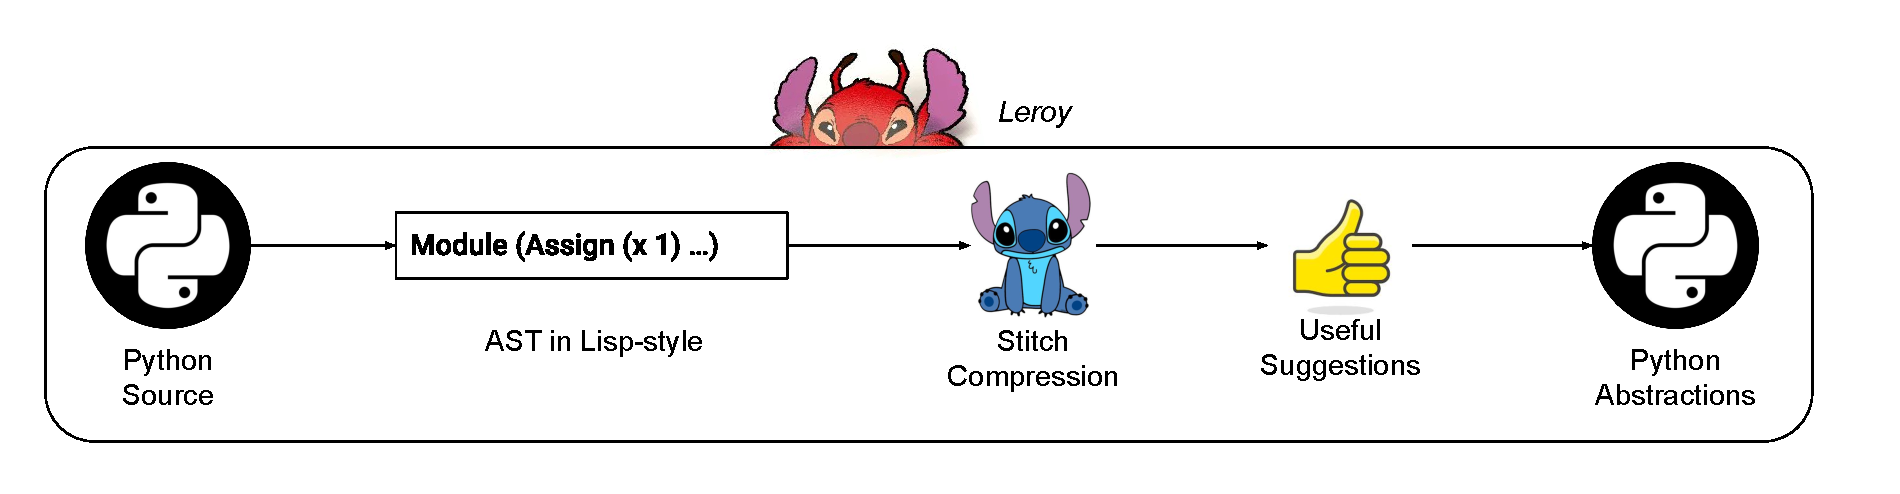
\includegraphics[width=\textwidth]{images/Design.pdf}
%   \caption{\toolname's high level design}
%   \label{fig:design}
% \end{figure*}
% \toolname performs library extraction by operating on the AST of the programming language. \toolname uses Stitch \cite{Bowers_2023stitch} as the library extraction engine, prunes invalid abstractions produced by it to present the most useful suggestions to the developer. Figure \ref{fig:design} shows the high level design of \toolname.
% % In the sections below, we describe each step in detail.

% \subsection{Representing Program AST in a lisp-like form}
% To convert program \textbf{ASTs to Lisp}, we treat ASTs as a series of nested function calls, with nodes as the function and subsequent child nodes as the argument of the function. This enables us to unwrap the AST into one long function call.
% % \todo{Add diagram of AST and converted lisp?}

% \subsection{Pruning Invalid Abstractions}
% Stitch suggests abstractions which involve language expressions/statements as function parameters. To \textbf{enhance abstractions} from stitch, we prune such cases. 


% \subsubsection{Macro-Like Abstractions}
% To prune macro-like abstractions, we attempt to convert the abstraction back into a program AST, and check if the tree is well-formed (all required children of a parent exist). Any incomplete ASTs are deemed to be macro-like and are pruned.

% \subsubsection{Invalid Parameters}
% We use a similar approach to find cases where invalid parameters could be passed to the abstraction. We convert the abstraction's body into a program AST and encode the abstraction's parameters as identifier nodes. 
% Then, we check if these identifier nodes are valid children in the AST. For example, an identifier node cannot be a valid child of a comparison expression's operator. But, an identifier node can be a valid child of the same expression's operand. 

% To summarise, if the AST is invalid or not well-formed, we deem the abstraction to be invalid.

% \subsection{Presenting Non-trivial Abstractions}

% To prune trivial abstractions (e.g. a function which performing addition of two arguments), we introduce a minimum size for the abstraction. This ensures that we have interesting abstractions coming out of \toolname.


% \subsection{Figuring out the return value}

% We augment the abstraction from Stitch by adding a necessary return value, if it does not exist. Our approach returns the last variable or expression in the abstraction's body. This is a simple approach that ensures that abstractions are functional in the target programming language. 

% % We remove abstractions which take language expressions/statements as parameters. 

% % \todo{This is the research problem. Add details when we have a more concrete solution.}

% % \subsection{Converting Lisp to Language AST}
% \subsection{Converting abstractions back to the PL}
% Finally, we convert the suggestions from stitch back into the AST. Then, we unparse the AST to result in the compressed code. 

% \todo{add design diagram.}
